% GNUPLOT: LaTeX picture with Postscript
\begingroup
  \makeatletter
  \providecommand\color[2][]{%
    \GenericError{(gnuplot) \space\space\space\@spaces}{%
      Package color not loaded in conjunction with
      terminal option `colourtext'%
    }{See the gnuplot documentation for explanation.%
    }{Either use 'blacktext' in gnuplot or load the package
      color.sty in LaTeX.}%
    \renewcommand\color[2][]{}%
  }%
  \providecommand\includegraphics[2][]{%
    \GenericError{(gnuplot) \space\space\space\@spaces}{%
      Package graphicx or graphics not loaded%
    }{See the gnuplot documentation for explanation.%
    }{The gnuplot epslatex terminal needs graphicx.sty or graphics.sty.}%
    \renewcommand\includegraphics[2][]{}%
  }%
  \providecommand\rotatebox[2]{#2}%
  \@ifundefined{ifGPcolor}{%
    \newif\ifGPcolor
    \GPcolorfalse
  }{}%
  \@ifundefined{ifGPblacktext}{%
    \newif\ifGPblacktext
    \GPblacktexttrue
  }{}%
  % define a \g@addto@macro without @ in the name:
  \let\gplgaddtomacro\g@addto@macro
  % define empty templates for all commands taking text:
  \gdef\gplbacktext{}%
  \gdef\gplfronttext{}%
  \makeatother
  \ifGPblacktext
    % no textcolor at all
    \def\colorrgb#1{}%
    \def\colorgray#1{}%
  \else
    % gray or color?
    \ifGPcolor
      \def\colorrgb#1{\color[rgb]{#1}}%
      \def\colorgray#1{\color[gray]{#1}}%
      \expandafter\def\csname LTw\endcsname{\color{white}}%
      \expandafter\def\csname LTb\endcsname{\color{black}}%
      \expandafter\def\csname LTa\endcsname{\color{black}}%
      \expandafter\def\csname LT0\endcsname{\color[rgb]{1,0,0}}%
      \expandafter\def\csname LT1\endcsname{\color[rgb]{0,1,0}}%
      \expandafter\def\csname LT2\endcsname{\color[rgb]{0,0,1}}%
      \expandafter\def\csname LT3\endcsname{\color[rgb]{1,0,1}}%
      \expandafter\def\csname LT4\endcsname{\color[rgb]{0,1,1}}%
      \expandafter\def\csname LT5\endcsname{\color[rgb]{1,1,0}}%
      \expandafter\def\csname LT6\endcsname{\color[rgb]{0,0,0}}%
      \expandafter\def\csname LT7\endcsname{\color[rgb]{1,0.3,0}}%
      \expandafter\def\csname LT8\endcsname{\color[rgb]{0.5,0.5,0.5}}%
    \else
      % gray
      \def\colorrgb#1{\color{black}}%
      \def\colorgray#1{\color[gray]{#1}}%
      \expandafter\def\csname LTw\endcsname{\color{white}}%
      \expandafter\def\csname LTb\endcsname{\color{black}}%
      \expandafter\def\csname LTa\endcsname{\color{black}}%
      \expandafter\def\csname LT0\endcsname{\color{black}}%
      \expandafter\def\csname LT1\endcsname{\color{black}}%
      \expandafter\def\csname LT2\endcsname{\color{black}}%
      \expandafter\def\csname LT3\endcsname{\color{black}}%
      \expandafter\def\csname LT4\endcsname{\color{black}}%
      \expandafter\def\csname LT5\endcsname{\color{black}}%
      \expandafter\def\csname LT6\endcsname{\color{black}}%
      \expandafter\def\csname LT7\endcsname{\color{black}}%
      \expandafter\def\csname LT8\endcsname{\color{black}}%
    \fi
  \fi
  \setlength{\unitlength}{0.0500bp}%
  \begin{picture}(15306.00,10204.00)%
    \gplgaddtomacro\gplbacktext{%
      \csname LTb\endcsname%
      \put(1210,704){\makebox(0,0)[r]{\strut{} 0}}%
      \put(1210,2243){\makebox(0,0)[r]{\strut{} 1e+06}}%
      \put(1210,3782){\makebox(0,0)[r]{\strut{} 2e+06}}%
      \put(1210,5322){\makebox(0,0)[r]{\strut{} 3e+06}}%
      \put(1210,6861){\makebox(0,0)[r]{\strut{} 4e+06}}%
      \put(1210,8400){\makebox(0,0)[r]{\strut{} 5e+06}}%
      \put(1210,9939){\makebox(0,0)[r]{\strut{} 6e+06}}%
      \put(1342,484){\makebox(0,0){\strut{} 0}}%
      \put(3603,484){\makebox(0,0){\strut{} 200}}%
      \put(5864,484){\makebox(0,0){\strut{} 400}}%
      \put(8126,484){\makebox(0,0){\strut{} 600}}%
      \put(10387,484){\makebox(0,0){\strut{} 800}}%
      \put(12648,484){\makebox(0,0){\strut{} 1000}}%
      \put(14909,484){\makebox(0,0){\strut{} 1200}}%
      \put(176,5321){\rotatebox{-270}{\makebox(0,0){\strut{}Kanalzahl}}}%
      \put(8125,154){\makebox(0,0){\strut{}Energie [MeV]}}%
      \put(2292,9016){\makebox(0,0)[l]{\strut{}Aufgabe 5.4}}%
      \put(2292,8796){\makebox(0,0)[l]{\strut{}Fitgleichung: Summe von}}%
      \put(2292,8576){\makebox(0,0)[l]{\strut{}Quadratischem Hintergrund $ax^2+bx+c$ mit $a=0.00734$, $b=-7.26$, $c=4370.0$}}%
      \put(2292,8356){\makebox(0,0)[l]{\strut{}Lorentzian $frac{a}{1+left(frac{x-p}{f/2}
ight)^2}$ mit $p=61.59$, $a=43480.0$, $f=-15.82$}}%
      \put(2292,8136){\makebox(0,0)[l]{\strut{}Lorentzian $frac{a}{1+left(frac{x-p}{f/2}
ight)^2}$ mit $p=295.4$, $a=27790.0$, $f=86.86$}}%
      \put(2292,7916){\makebox(0,0)[l]{\strut{}Lorentzian $frac{a}{1+left(frac{x-p}{f/2}
ight)^2}$ mit $p=530.2$, $a=37690.0$, $f=17.21$}}%
      \put(2292,7696){\makebox(0,0)[l]{\strut{}Lorentzian $frac{a}{1+left(frac{x-p}{f/2}
ight)^2}$ mit $p=631.2$, $a=31100.0$, $f=16.41$}}%
      \put(2292,7476){\makebox(0,0)[l]{\strut{}Lorentzian $frac{a}{1+left(frac{x-p}{f/2}
ight)^2}$ mit $p=710.2$, $a=24500.0$, $f=11.73$}}%
      \put(2292,7256){\makebox(0,0)[l]{\strut{}Lorentzian $frac{a}{1+left(frac{x-p}{f/2}
ight)^2}$ mit $p=775.3$, $a=20580.0$, $f=10.91$}}%
      \put(2292,7036){\makebox(0,0)[l]{\strut{}Lorentzian $frac{a}{1+left(frac{x-p}{f/2}
ight)^2}$ mit $p=832.6$, $a=17310.0$, $f=10.54$}}%
      \put(2292,6816){\makebox(0,0)[l]{\strut{}Lorentzian $frac{a}{1+left(frac{x-p}{f/2}
ight)^2}$ mit $p=884.5$, $a=14970.0$, $f=9.653$}}%
      \put(2292,6596){\makebox(0,0)[l]{\strut{}Lorentzian $frac{a}{1+left(frac{x-p}{f/2}
ight)^2}$ mit $p=931.9$, $a=13240.0$, $f=8.975$}}%
      \put(2292,6376){\makebox(0,0)[l]{\strut{}Lorentzian $frac{a}{1+left(frac{x-p}{f/2}
ight)^2}$ mit $p=976.0$, $a=11280.0$, $f=8.229$}}%
      \put(2292,6156){\makebox(0,0)[l]{\strut{}Lorentzian $frac{a}{1+left(frac{x-p}{f/2}
ight)^2}$ mit $p=1018.0$, $a=9241.0$, $f=8.559$}}%
    }%
    \gplgaddtomacro\gplfronttext{%
    }%
    \gplbacktext
    \put(0,0){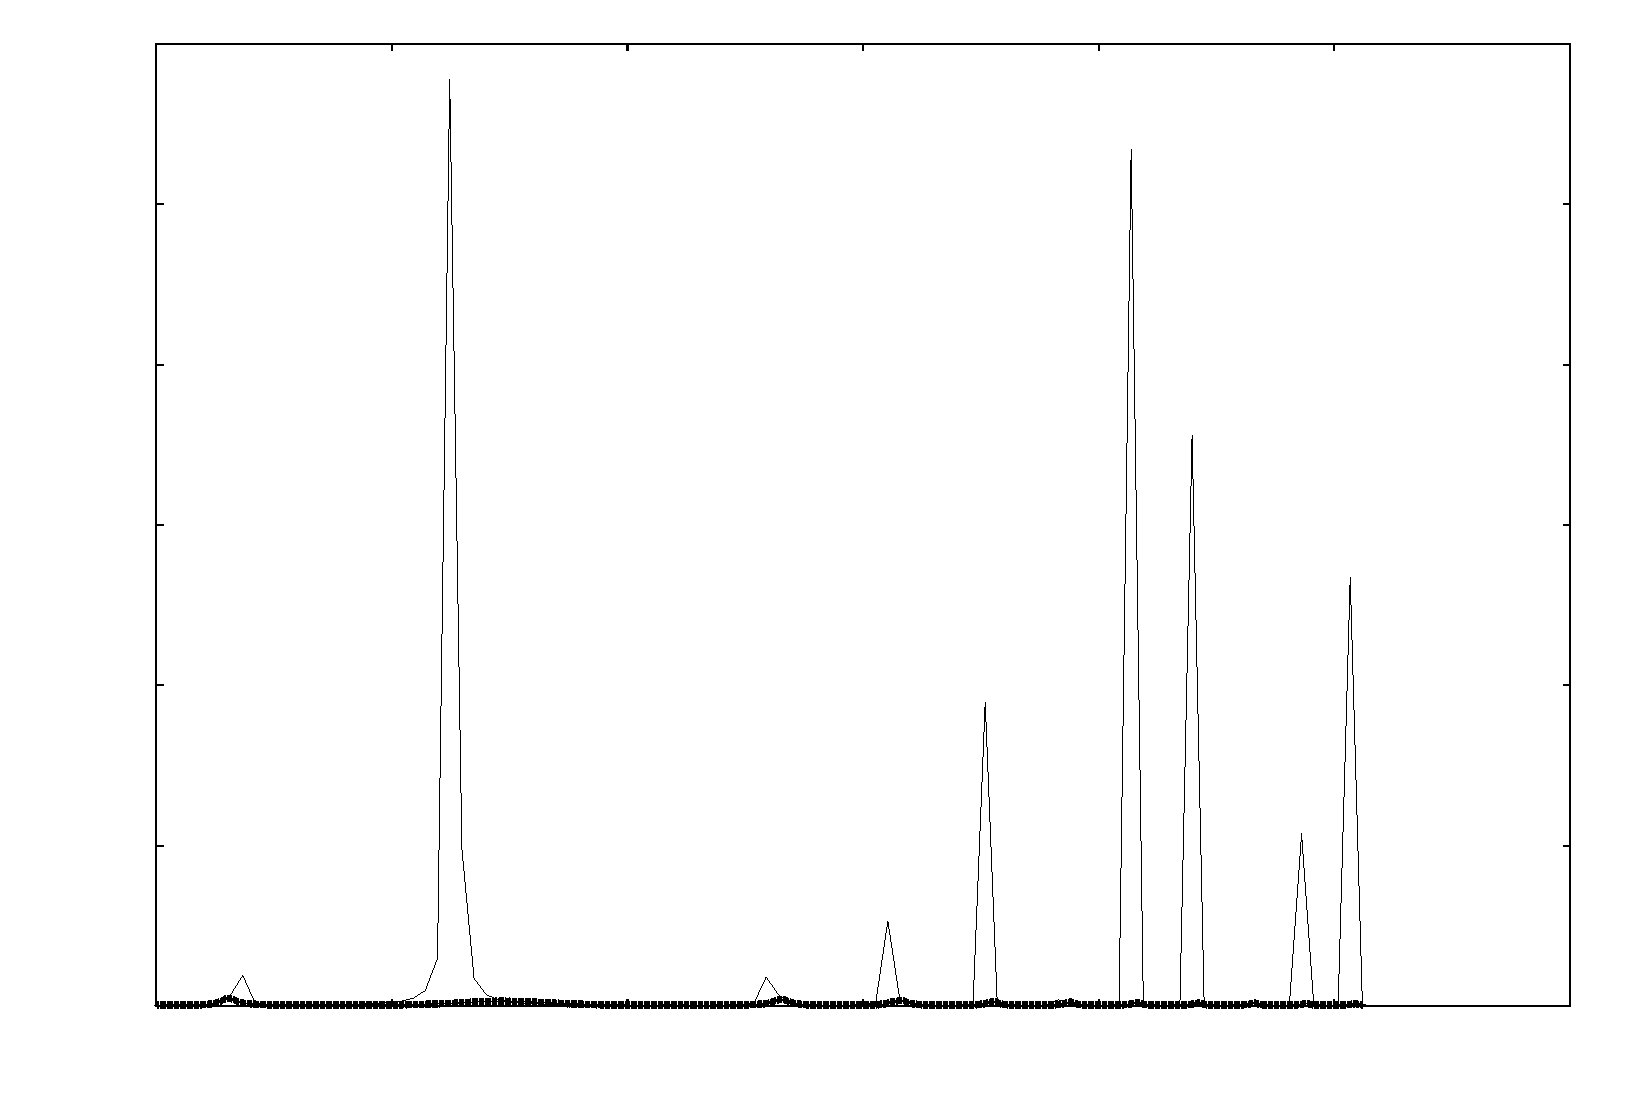
\includegraphics{plot-1}}%
    \gplfronttext
  \end{picture}%
\endgroup
